\documentclass[11pt,a4paper]{article}
\usepackage[utf8]{inputenc}
\usepackage[T1]{fontenc}
\usepackage[french]{babel}
\usepackage[margin=1.5cm]{geometry}
\usepackage{graphicx}
\usepackage{hyperref}
\usepackage{enumitem}
\usepackage{titlesec}

\setlist{nosep,leftmargin=1.2em}
\titlespacing*{\section}{0pt}{0.4em}{0.2em}
\titleformat{\section}{\normalfont\bfseries\large}{\thesection}{0.5em}{}
\setlength{\parskip}{0.2em}
\setlength{\parindent}{0pt}

\title{\vspace{-1.5cm}Rapport individuel --- It\'eration 1}
\author{Mati Afriat (\texttt{mat6784}) --- Projet Long SHDL}
\date{13 avril 2026}

\begin{document}
\maketitle
\vspace{-2em}

\section*{Contexte}
Responsable du \textbf{simulateur de circuits logiques} (axe \emph{simulation}, branche \texttt{simulation}). Objectif sprint~1~: poser un mod\`ele objet capable de repr\'esenter portes combinatoires et bascules s\'equentielles, calculer leur \'etat ternaire (\texttt{UP}/\texttt{DW}/\texttt{ND}) et propager les valeurs jusqu'\`a stabilisation. Exploration de deux mod\'elisations en parall\`ele avant de choisir celle qui sera maintenue.

\section*{Activit\'es r\'ealis\'ees}
\begin{itemize}
  \item \textbf{Mod\'elisation par Lien} (\texttt{tests projet long/simulateur/})~: fil \texttt{Lien} portant un \texttt{Etat \{UP, DW, ND\}}, composants abstraits avec entr\'ees/sorties (\texttt{And}, \texttt{Or}, \texttt{Non}, \texttt{Duplicateur}, \texttt{Porte}), regroupement par \texttt{TableauLien} et \texttt{Module}.
  \item \textbf{Bascules s\'equentielles}~: \texttt{Bascule}, \texttt{BasculeD}, \texttt{BasculeClock} valid\'ees par les scripts \texttt{testBascule}/\texttt{testBasculeD}/\texttt{testBasculeClock}.
  \item \textbf{Moteur de simulation}~: \texttt{File}/\texttt{FileListe} pour l'ordonnancement des recalculs.
  \item \textbf{Mod\'elisation alternative par Connecteur} (\texttt{simulateur/})~: interfaces \texttt{Connecteur}/\texttt{Composant}/\texttt{Structure}, \texttt{DicoConnecteur}, \texttt{LienVecteur}, \texttt{Multiplicateur}, \texttt{BouttonEntree}. Approche plus abstraite pens\'ee pour les vecteurs et la composition.
\end{itemize}

\section*{R\'esultats}
\begin{itemize}
  \item \textbf{Mod\`ele Lien fonctionnel}~: 5 classes test\'ees en JUnit (\texttt{AndTest}, \texttt{OrTest}, \texttt{NonTest}, \texttt{LienTest}, \texttt{TableauLienTest}, \texttt{DuplicateurTest}), bascule D valid\'ee par un script de table de v\'erit\'e.
  \item \textbf{18 fichiers Java} dans \texttt{simulateur/} (approche Connecteur) + \textbf{27 fichiers Java} dans \texttt{tests projet long/simulateur/} (approche Lien).
  \item Le mod\`ele Lien est jug\'e suffisant pour le sprint~2 sur la combinatoire scalaire~; l'approche Connecteur reste comme piste pour les vecteurs et l'appel de module.
\end{itemize}

\begin{center}
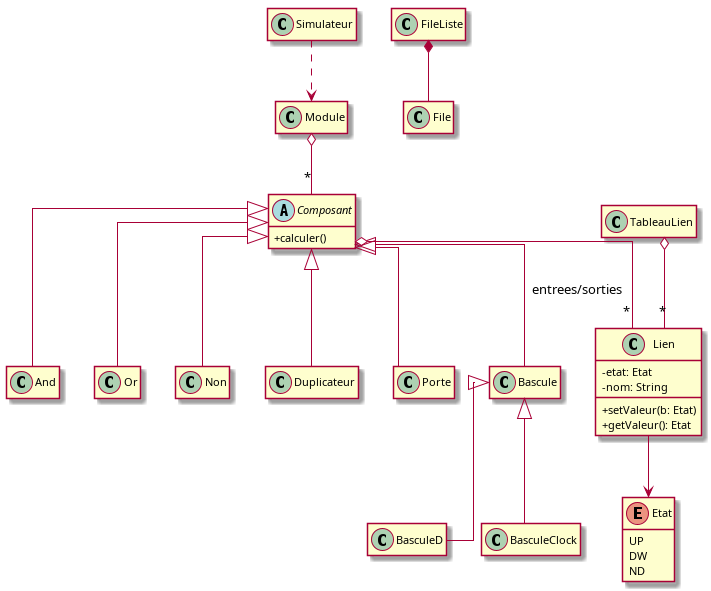
\includegraphics[width=0.42\textwidth]{../mati-sprint1-classes.png}\\
{\small Figure --- Diagramme de classes du mod\`ele Lien (source \texttt{mati-sprint1-classes.puml}).}
\end{center}

\section*{Difficult\'es et r\'eussites}
Difficult\'e~: la \textbf{convergence des circuits s\'equentiels}. Les bascules introduisent des boucles de r\'etroaction~; il a fallu d\'efinir un ordre de recalcul stable et un \'etat \texttt{ND} pour les liens non encore d\'efinis, ce qui a guid\'e le choix de la file d'\'ev\'enements. R\'eussite~: la base combinatoire est tr\`es simple \`a tester et a servi de socle pour les bascules sans modification ult\'erieure.

\section*{Manuel utilisateur}
Pr\'e-requis~: JDK~21+, JUnit~4 et Hamcrest. Tests~: \texttt{javac -cp lib/junit-4.13.2.jar:lib/hamcrest-core-1.3.jar 'tests projet long/simulateur/*.java'} puis \texttt{java org.junit.runner.JUnitCore simulateur.AndTest}. Scripts de bascule~: \texttt{java simulateur.testBasculeD}. Code sur la branche \texttt{simulation}.

\end{document}
